\section{Matrix Multiplication Implementation}

Matrix multiplication can be done sequentially on the CPU in time complexity $O(l \cdot m \cdot n)$, where matrix $\mathbf{A}$ is $l*m$, matrix $\mathbf{B}$ is $m*n$ and the result matrix $\mathbf{C}$ is $l*n$. For square matrices this can be expressed as $O(n^3)$ for $n^2$ data. For each element to be computed, $O(n)$ many independent arithmetic operations have to be performed. Because these operations are independent, they can be computed in parallel. This can potentially have a large positive impact on performance.

\subsection{Multiplication: CPU}

The implementation follows a standard sequential procedure with a triple nested for-loop. For each element in the output matrix, a row from input matrix $\mathbf{A}$ is paired with a column from input matrix $\mathbf{B}$ as illustrated in Figure \ref{fig:multiplication_illustration}.  In this implementation, a single CPU core will compute the entire result matrix.

\begin{lstlisting}[language=C, caption={Matrix Multiplication on the CPU}, label={lst:matrix_multiplication_cpu}]
bool matrix_multiplication(matrix_t *matrix_a, matrix_t *matrix_b, matrix_t *matrix_c) {
    // input validation and variable declarations { ... }
    for (int i = 0; i < result_rows; i++)
        for (int j = 0; j < result_columns; j++) {
            sum_of_products = 0.0f;
            for (int k = 0; k < common_dimension_length; k++) // consider renaming to m
                sum_of_products +=
                    matrix_a->values[INDEX(i, k, matrix_a_columns)] *
                    matrix_b->values[INDEX(k, j, matrix_b_columns)];
            matrix_c->values[INDEX(i, j, result_columns)] = sum_of_products;
        }
    return true;
}
\end{lstlisting}

As can be seen in figure \ref{fig:mul_cpu_bench}, the slope of the CPU implementation's running time is $\sim 3$. This is expected, since the algorithms time complexity is $O(n^3)$ for square matrices.

\subsection{Multiplication: GPU Single Core}

The same procedure is implemented on the GPU, to compare the single core version from the CPU with the GPU. This kernel is launched with a block size and grid size of 1, making it run on a single core.

\begin{lstlisting}[language=C, caption={Matrix Multiplication on the gpu}, label={lst:matrix_multiplication_gpu}]
__global__ void cuda_matrix_multiplication_single_core_kernel(
    device_matrix_t matrix1, device_matrix_t matrix2, device_matrix_t result,
    int l, int n, int m) {
    float sum_of_products;

    for (int i = 0; i < l; i++)
        for (int j = 0; j < n; j++) {
            sum_of_products = 0.0f;
            for (int k = 0; k < m; k++)
                sum_of_products += matrix1[INDEX(i, k, m)] 
                    * matrix2[INDEX(k, j, n)];
            result[INDEX(i, j, n)] = sum_of_products;
        }
}
\end{lstlisting}

As can be seen in figure \ref{fig:mul_cpu_bench}, the single core implementation of matrix multiplication looks similar to the single core implementation of matrix addition. Again, this is likely due to the overhead of allocating memory on the GPU.

\begin{figure}[h]
  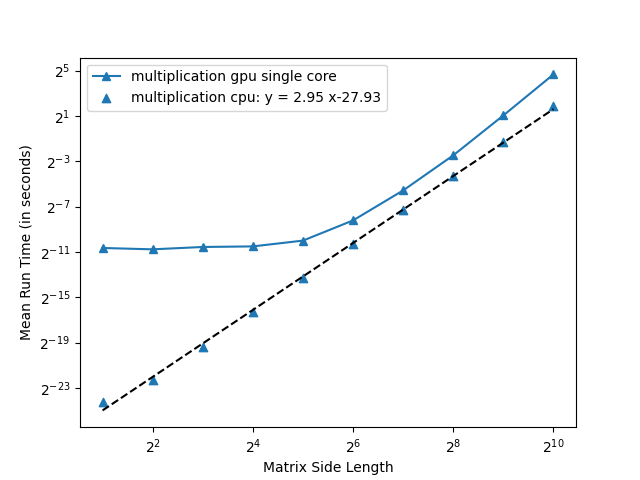
\includegraphics[width=.70\textwidth]{SavedBenchmarksAndDiagrams/Machine 2/Multiplication/CPU, GPU SC.png}
  \centering
  \caption{Multiplication: CPU And GPU Single Core Benchmark}
  \label{fig:mul_cpu_bench}
\end{figure}

Notably, the lines are a lot closer than they were with addition. This is likely due to the fact that matrix multiplication has a cubic time complexity, whereas matrix addition is quadratic, meaning the overhead has less of an impact. In other words, with matrix multiplication the GPU is able to more easily "catch-up" to the CPU implementation, since the CPU implementation is slower.

At the end of our benchmarks, the slope of our single core GPU implementation seems to grow steeper. From the results seen in figure \ref{fig:diagnostic_benchmark}, this increase is likely due to the amount of data we have to copy back and forth between the CPU and GPU.

The following three sections will explore various approaches to improve runtime performance by utilizing the GPU architecture in different ways.

\subsection{Multiplication: GPU Multi Core Unwrapping i}

To utilize the block architecture of the GPU, we initialize our grid to be one-dimensional with $l$ many blocks, where $l$ is the number of rows in the result matrix. Each block has a single thread.

One thread (and block) is then responsible for computing one column of the result matrix. This essentially \textit{unwraps} the outermost for-loop (using i as the counter), which was previously iterating over all rows. Therefore this implementation is dubbed "unwrapping i". One is then left with a nested for-loop, as can be seen in listing \ref{lst:matrix_multiplication_gpu_multi_core}.

\begin{lstlisting}[language=C, caption={Multi Core Matrix Multiplication "Unwrapping $i$"}, label={lst:matrix_multiplication_gpu_multi_core}]
__global__ void cuda_matrix_multiplication_multicore_unwrapping_i_kernel(
    device_matrix_t matrix_a, device_matrix_t matrix_b,
    device_matrix_t matrix_c, int l, int n, int m) {

    int i = blockIdx.x;
    float sum_of_products;
    for (int j = 0; j < n; j++) {
        sum_of_products = 0.0f;
        for (int k = 0; k < m; k++)
            sum_of_products += matrix_a[INDEX(i, k, m)] 
                * matrix_b[INDEX(k, j, n)];
        matrix_c[INDEX(i, j, n)] = sum_of_products;
    }
}
\end{lstlisting}

\begin{figure}[h]
  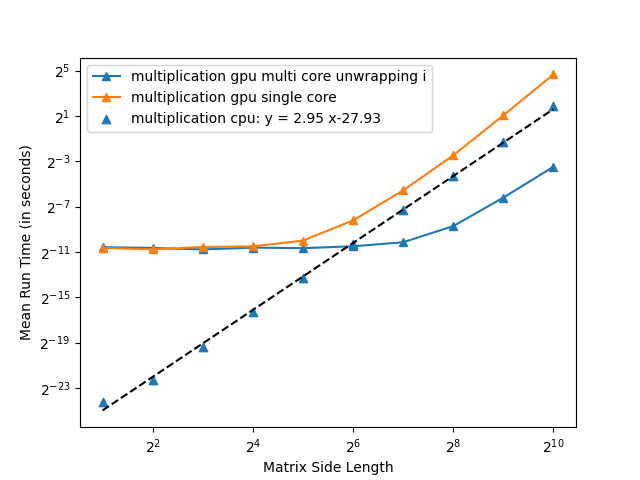
\includegraphics[width=0.5\textwidth]{SavedBenchmarksAndDiagrams/Machine 2/Multiplication/GPU MC Unwrap i.png}
  \centering
  \caption{Multiplication: GPU "Unwrap $i$"}
  \label{fig:mul_unwrap_i_bench}
\end{figure}

As can be seen figure \ref{fig:mul_unwrap_i_bench}, this implementation is actually faster than the CPU implementation. The running times stay constant for a long time. When they rise, it is likely due to the amount of data that has to be copied back and forth.

\subsection{Multiplication: GPU Multi Core Unwrapping i and j}

Taking this one step further, we will now utilize that each block can have many threads. Specifically, we will spawn $n$ many threads in each block, where $n$ is the number of columns in the result matrix. 

This way, each thread will be responsible for computing a single element of the result matrix. The block determines which row and the thread determines which column. This leaves us with a kernel that has only a single for loop as can be seen in listing \ref{lst:matrix_multiplication_gpu_multi_core_multi_thread}. 

\begin{lstlisting}[language=C, caption={Multi Core "Unwrapping $i$ and $j$"}, label={lst:matrix_multiplication_gpu_multi_core_multi_thread}]
__global__ void cuda_matrix_multiplication_unwrapping_i_and_j_kernel(
    device_matrix_t matrix_a, device_matrix_t matrix_b,
    device_matrix_t matrix_c, int l, int n, int m) {
    int i = blockIdx.x;
    int j = threadIdx.x;
    float sum_of_products = 0.0f;

    for (int k = 0; k < m; k++)
        sum_of_products += matrix_a[INDEX(i, k, m)] 
            * matrix_b[INDEX(k, j, n)];

    matrix_c[INDEX(i, j, n)] = sum_of_products;
}
\end{lstlisting}

As seen in figure \ref{fig:mul_unwrap_i_and_j_bench}, the unwrapping of both $i$ and $j$ results in even faster running times. This is likely due to the fact that each thread has less work to do, and more threads will be utilized at once because of this.

\begin{figure}[h]
  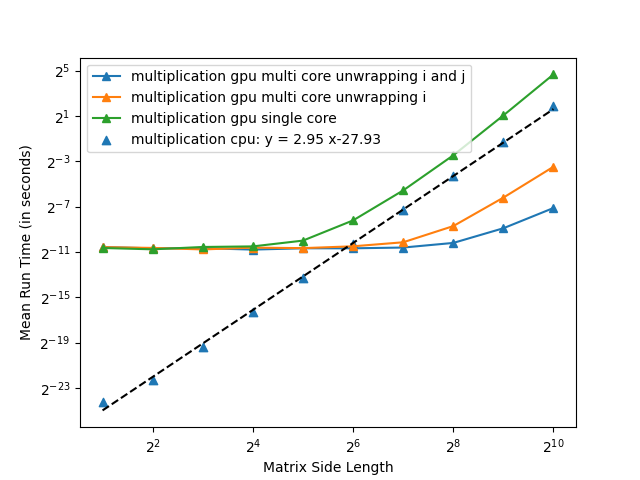
\includegraphics[width=0.5\textwidth]{SavedBenchmarksAndDiagrams/Machine 2/Multiplication/GPU MC Unwrap i, j.png}
  \centering
  \caption{Multiplication: GPU "Unwrap $i$ and $j$".}
  \label{fig:mul_unwrap_i_and_j_bench}
\end{figure}

Like the first addition multi core implementation, we face the limitation that the maximum block size is 1024, meaning if we try to compute a matrix multiplication where $n$ is greater than 1024, it simply will not work. Our next section will rectify this limitation.

\subsection{Multiplication: GPU Multi Core Shared Memory}

% Reference Variable Memory Space Specifiers: https://docs.nvidia.com/cuda/cuda-c-programming-guide/index.html#variable-memory-space-specifiers

In matrix multiplication, each computed element in matrix $\mathbf{C}$ requires $m$ many reads from matrix $\mathbf{A}$ and $m$ many reads from matrix $\mathbf{B}$. Computing the full ${n \cdot l}$ matrix $\mathbf{C}$ then requires $2m \cdot n \cdot l$ many reads. For each time we want to access an element from $\mathbf{B}$ or $\mathbf{C}$ we have to query the L2 cache or (in the event of a cache miss) the global VRAM. This is a potential bottleneck to the algorithm. To alleviate this, we wish to use the faster L1 cache that can be shared across a block. Even though the L1 cache is very fast, it is also very limited in size and only avaiable between the threads of a single block. 

The following implementation is strongly inspired by \cite[Sect. 3.2.4]{nvidia:cudadoc}. It aims to better utilize the memory architecture on the GPU. 

The key observation is that each element in matrix $\mathbf{A}$ will be accessed $n$ many times, and each element in matrix $\mathbf{B}$ will be accessed $l$ many times. This implementation will take advantage of the fact that an element is needed many times by storing them in the very fast L1 cache. 

For this implementation, each thread will still only be responsible for calculating a single element in the result matrix. However, our blocks will be defined by threads, that access much of the same memory. These threads will help each other retrieve the commonly accessed values from matrix $\mathbf{A}$ and $\mathbf{B}$. By doing this, the L1 cache is filled in parallel with the commonly accessed memory, so that all threads can quickly access it and compute their values. 

To fit the memory we want to access into the L1 cache, we will divide the matrices into submatrices (see figure \ref{fig:matrix_shared_memory}). We tried using different values for \texttt{block\_size} (the unit we divide the submatrices with), and eventually landed on 16 as a sweet-spot.

\begin{figure}[h]
    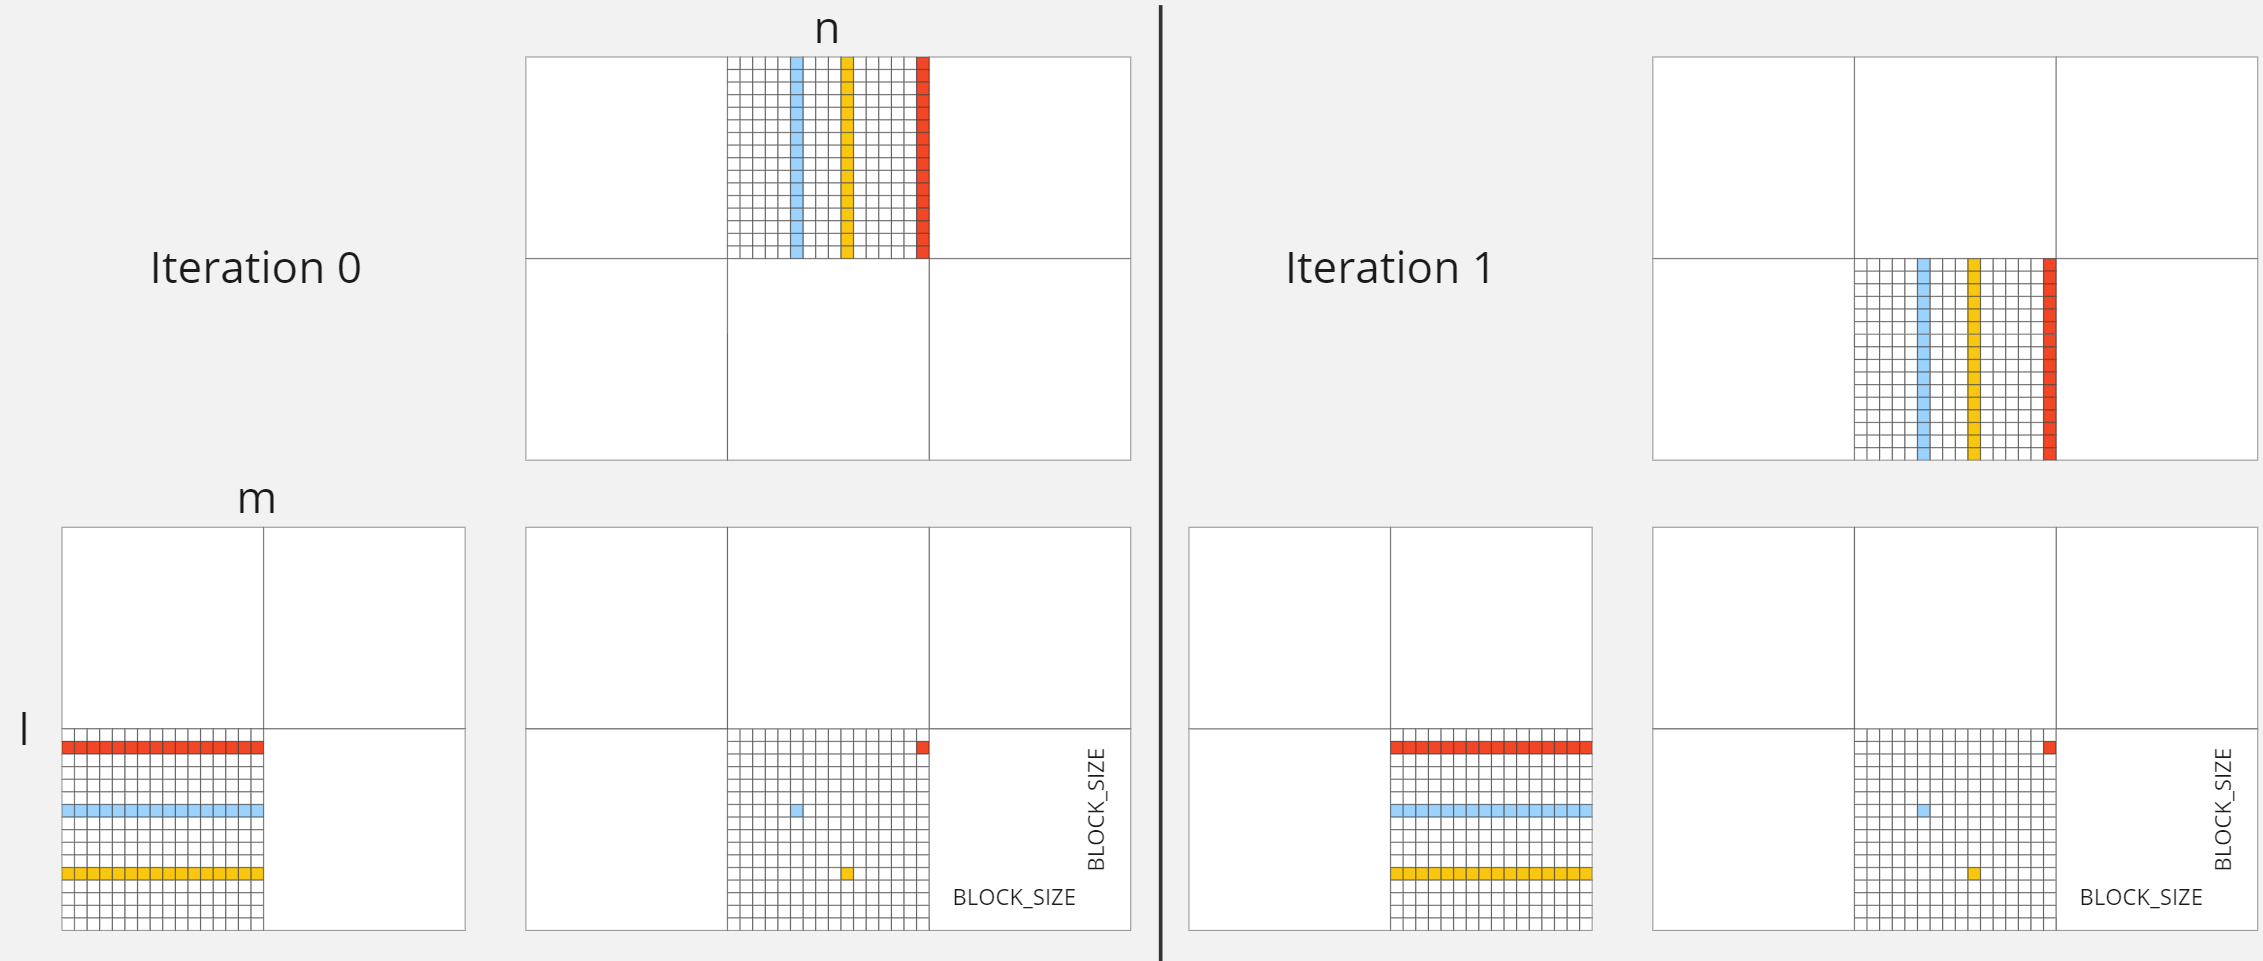
\includegraphics[width=\textwidth]{Documents/Report/Figures/SharedMemory.png}
    \centering
    \caption{The submatrices are tiled according to blocksizes and accessed in each iteration as shown.}
    \label{fig:matrix_shared_memory}
\end{figure}

This means that a single block will put 16 by 16 floats in their shared cache. This comes out to 256 floats of 4 bytes each meaning 1024 bytes or 1 KB. On our bench machine, the graphics card has an L1 cache of 128 KB (per SM), so one might think that such a small block size is wasteful. After all, we could have 128x larger submatrices, and still have them fit in the L1 cache.

However, each SM may run multiple blocks at once, meaning they will take as many blocks as they can fit. We aim to write code that runs well on many different machines, meaning we would rather have many smaller blocks, rather than a few large blocks, since it scales better with older or lower-end graphic cards with more limited L1 caches.

In CUDA we access the L1 cache with the \textit{shared memory} specifier \cite[Sect. 7.2.3]{nvidia:cudadoc}. It is called shared memory, because it is shared between the threads inside the block.\\

\noindent Previously we have only accessed our blocks and threads by their x-coordinate. For this implementation, it helps to abstract the memory access to be 2-dimensional. That means we will start to access our specific blocks and threads with both x- and y-coordinates. 

Now that we have tiled our blocks to cover the grid, we will concentrate on a single arbitrary block. This block has $16 \cdot 16$ many threads. Each block will have 2 corresponding sub matrices, also of size $16 \cdot 16$. These will be declared as \texttt{\_\_shared\_\_} float 2D-arrays. This keyword in CUDA tells the compiler to put this memory on the shared L1 cache, such that all threads within the block has access to it. 

The next step of the algorithm is to loop through $m / 16$ many squares of matrix $\mathbf{A}$ and matrix $\mathbf{B}$. In reality, it will be $(m + 15) / 16$, to introduce some padding for matrices that do not evenly divide into 16. For each iteration, each thread will write one value from $\mathbf{A}$ and $\mathbf{B}$ to these shared matrices. With these in place, each thread can now sum up 16 many products. Doing this in $m / 16$ many iterations will allow each thread to calculate the full matrix product and store the result in matrix $\mathbf{C}$. 

To avoid race conditions, we use the CUDA method \texttt{\_\_syncthreads} to synchronize the threads. In each iteration it is called first to make sure all values of matrix $\mathbf{A}$ and $\mathbf{B}$ are retrieved before using them for calculations. It is called one more time to ensure all threads are done using the values before they are overwritten again for the next iteration. See the implementation in listing \ref{lst:matrix_multiplication_gpu_shared_memory}. 

\begin{lstlisting}[language=C, caption={Shared Memory Matrix Multiplication}, label={lst:matrix_multiplication_gpu_shared_memory}]
__global__ void cuda_matrix_multiplication_multi_core_shared_memory_kernel(
    device_matrix_t matrix_a, device_matrix_t matrix_b,
    device_matrix_t matrix_c, int l, int n, int m) {
    
    int block_row = blockIdx.y;
    int block_column = blockIdx.x;
    int row = threadIdx.y;
    int column = threadIdx.x;
    float c_value = .0f;

    int subs_in_m = (m + BLOCK_SIZE - 1) / BLOCK_SIZE;
    for (int k = 0; k < subs_in_m; k++) {
        device_matrix_t a_sub = get_sub_matrix(matrix_a, block_row, k, m);
        __shared__ float shared_a_sub[BLOCK_SIZE][BLOCK_SIZE];
        shared_a_sub[row][column] = a_sub[INDEX(row, column, m)];

        device_matrix_t b_sub = get_sub_matrix(matrix_b, k, block_column, n);
        __shared__ float shared_b_sub[BLOCK_SIZE][BLOCK_SIZE];
        shared_b_sub[row][column] = b_sub[INDEX(row, column, n)];
        __syncthreads();

        for (int i = 0; i < BLOCK_SIZE; i++) 
            c_value += shared_a_sub[row][i] * shared_b_sub[i][column];
        __syncthreads();
    }

    if (row + BLOCK_SIZE * block_row < l && column + BLOCK_SIZE * block_column  < n) {
        device_matrix_t c_sub = get_sub_matrix(matrix_c, block_row, block_column, n);
        c_sub[INDEX(row, column, n)] = c_value;
    } 
}
\end{lstlisting}

As can be seen in figure \ref{fig:mul_all_bench}, the shared memory implementation only becomes marginally faster with very large matrices. Because our "unwrapping $i$ and $j$" implementation only works up to 1024, we do not know if it would much faster with even larger martrices, but judging from our results, it seems likely.

\begin{figure}[h]
  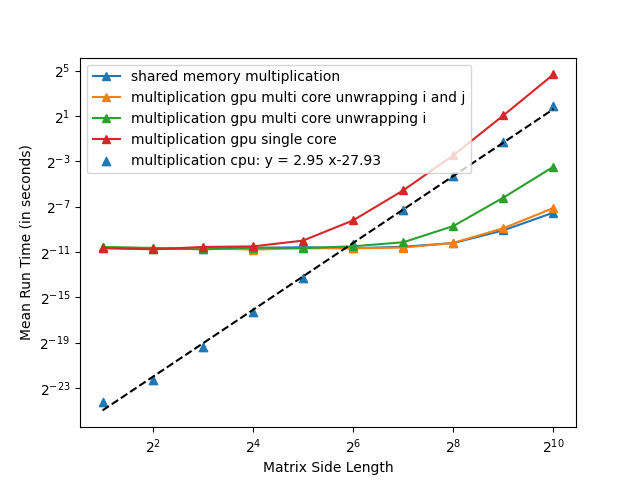
\includegraphics[width=\textwidth]{SavedBenchmarksAndDiagrams/Machine 2/Multiplication/GPU Shared 1.png}
  \centering
  \caption{Multiplication: All benchmarks.}
  \label{fig:mul_all_bench}
\end{figure}

% Define shared A sub and B sub
% Define how they move across matrix C in m / block_size iterations, moving shared subs for every iteration
% Explain how in each iteration, one thread retrives one value from global memory/DRAM L2 and puts it in local memory/L1
% When shared sub a and b are filled out, (sync threads), each thread's c_value is added to
% When shared a and b have moved all the way through m, c_value is calculated and can be stored in global memory.

